The amount of keywords you have in a \app{} test and the amount of components your test deals with can grow very quickly. For this reason, it is important to think about structuring the \gdtestcasebrowser{} and the \gdomeditor{} to make finding \gdcases{} and component names easier. 


\subsection{Opening items in editors}
\gdhelpid{testCaseOpenExistingContextId}{Open Existing Test Case}
\gdhelpid{testExecViewContextId}{Test Suite Browser}
\gdhelpid{testSpecificationViewContextId}{Test Case Browser}
To open an existing \gdcase{}, \gdsuite{} or \gdjob{} in an editor, you can either double-click the item you want to open in its browser or you can select:\\
\bxmenu{Open With}{... Editor}{}\\
from the context-sensitive menu for the item. 

You can also open an existing \gdcase{} without having to select it from the \gdtestcasebrowser{} using the \bxname{Open Test Case} dialog \bxpref{TasksOpenExistingTC}. 





\subsection{Adding items to editors}
\gdhelpid{guidancerSpecTestCaseEditorContextId}{Test Case Editor}
\gdhelpid{testSpecificationViewContextId}{Test Case Browser}
\gdhelpid{testCaseAddExistingContextId}{Existing Test Case Dialog}
\gdhelpid{testSuiteEditorContextId}{Test Suite Editor}
\gdhelpid{testExecViewContextId}{Test Suite Browser}
\gdhelpid{guidancerTestJobEditorContextId}{Test Job Editor}
\label{TasksEditorAdd}
\index{Event Handler!Add}
\index{Add!Event Handler}



This section deals with adding \gdehandlers{} to \gdcases{}.  For information on using \gdehandlers{} meaningfully to ensure that your test execution is as robust as possible, see the section on \gdehandlers{} in the Best Practices section \bxpref{BPEHandlers}. 

\begin{enumerate}
\item Open the \gdtestcaseeditor{} by double-clicking on the \gdcase{} you want to edit in the \gdtestcasebrowser{}.   
\item Select\\
\bxmenu{Add}{\gdcase{} as \gdehandler{}}{} \\from the context-sensitive menu in the editor or use \bxkey{Ctrl+Enter}. 

\bxtipp{You can also drag the \gdcase{} you want to use straight into the \gdehandlers{} area of at the bottom of th the \gdtestcaseeditor{}. }

\item Choose a \gdcase{} to add from the dialog that appears.
\bxtipp{You can't add a \gdcase{} to itself as an \gdehandler{}, because this would create an infinite loop. }
\item Select an event type from the combo box \bxpref{eventtype}.
\item Select a reentry type from the combo box \bxpref{reentrytype}. 
\bxtipp{For each \gdcase{} you can only add one \gdehandler{} for each event type.}
\item Click \bxcaption{OK}. 
\item The \gdehandler{} appears in the lower half of the \gdtestcaseeditor{}. 
\gdmarpar{../../../share/PS/EventHandler}{ \gdehandler{}}
\item Save the changes in the editor.
\end{enumerate}



\subsection{Deleting items from editors}
\gdhelpid{guidancerSpecTestCaseEditorContextId}{Test Case Editor}
\gdhelpid{guidancerTestJobEditorContextId}{Test Job Editor}
\gdhelpid{testSuiteEditorContextId}{Test Suite Editor}
\label{TasksEditorDelete}
\index{Component!Names!Delete}
\index{Delete!Component Names}

When you reassign component names in the \gdcompnamesview{}, you automatically create new component names if the name you enter did not previously exist in the \gdproject{}. 

Larger \gdprojects{} can often end up with a number of component names that are no longer used. You can see and delete these names in the \gdcompnamebrowser{}. 
The names in the \bxname{Unused Component Names} category are not used anywhere in this \gdproject{} -- they are not present in any \gdcases{} and they have not been mapped to any technical names from the \gdaut{} in the \gdomeditor{} (\bxfigref{}). 

\begin{figure}[h]
\begin{center}
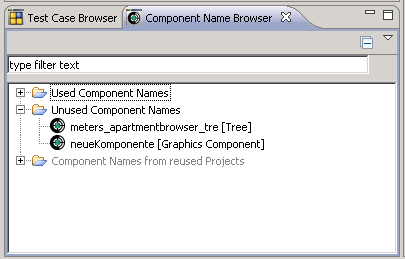
\includegraphics{Tasks/Compnames/PS/compnamebrowser}
\caption{The \gdcompnamebrowser{}}
\label{compnamebrowser}
\end{center}
\end{figure} 

To delete unused component names, select the name you want to delete and select:\\
\bxmenu{Delete}{}{}\\
from the context-menu. 



\subsection{Renaming items in editors}
\gdhelpid{guidancerTestJobEditorContextId}{Test Job Editor}
\gdhelpid{guidancerSpecTestCaseEditorContextId}{Test Case Editor}
\gdhelpid{testSuiteEditorContextId}{Test Suite Editor}
\label{TasksEditorRename}
\index{Test Case!Renaming}
\index{Renaming!Test Cases}
\index{Test Suite!Renaming}
\index{Renaming!Test Suites}
\index{Test Job!Renaming}
\index{Renaming!Test Jobs}
\index{Renaming!Component Names}
\index{Component Name!Renaming}

To rename an item in the \gdtestcasebrowser{}, \gdtestsuitebrowser{} or \gdcompnamebrowser{}:

\begin{enumerate}
\item Select the item you want to rename in the browser. 
\item Select:\\
\bxmenu{Rename}{}{}\\
from the context-sensitive menu. 
\item In the dialog which appears, enter a new name and click \bxcaption{OK}. 
\end{enumerate}

\bxtipp{You can also press \bxkey{F2} to rename an item.}

When you rename a \gdcase{} or \gdsuite{}, you change its specification name. 

If you have reused this \gdcase{} or \gdsuite{} in other \gdcases{}, \gdsuites{} or \gdjobs{}, the name will also be changed in the places where you have reused it but not renamed it. 



\subsection{Adding comments to items in editors}
\gdhelpid{guidancerSpecTestCaseEditorContextId}{Test Case Editor}
\gdhelpid{testSuiteEditorContextId}{Test Suite Editor}
\gdhelpid{guidancerTestJobEditorContextId}{Test Job Editor}
\label{TasksEditorAddComment}
\index{Add!Comments}
\index{Comment!Add}

You can add comments to items via the editor for an item. You can add comments to the item itself, or to other items used in it. 


\begin{enumerate}
\item Open the editor for the item you want to add comments to. 
\item Enter a comment in the \bxname{comment} field in the  \gdpropview{}. 
\item Save the changes
\item Comments can be overwritten when an item is reused.
\bxtipp{You can see the comment for a \gdcase{} when you hover over it in the \gdtestcasebrowser{} or the \gdtestsuitebrowser{} or in the search results view.}
\end{enumerate}

\bxtipp{You can also add comments to categories using the context-menu in the browser \bxpref{TasksCategoriesComment} and to the \gdproject{} itself via the \gdproject{} properties \bxpref{ProjPropertiesGeneral}.}


\subsection{Commenting out items in editors}
\gdhelpid{guidancerSpecTestCaseEditorContextId}{Test Case Editor}
\gdhelpid{testSuiteEditorContextId}{Test Suite Editor}
\label{TasksEditorDeactivate}
In the \gdtestcaseeditor{} and the \gdtestsuiteeditor{}, you can deactivate and reactivate \gdcases{} and \gdsteps{}. 

\begin{enumerate}
\item Select the \gdsteps{} or \gdcases{} you want to deactivate and select:\\
\bxmenu{Set as active / inactive}{}{}\\
from the context menu.
\bxtipp{You can also use \bxkey{ctrl+7} to toggle the items as active or inactive.}
\item The items you selected will be set as inactive. They are shown with green text and the sign \verb+//+ before the \gdcase{} or \gdstep{} name.
\item Any inactive items are not considered in \gdsuite{} validation, nor are they executed during a test run. 
\item You can reactivate the items by selecting:\\
\bxmenu{Set as active / inactive}{}{}\\
from the context menu.
\end{enumerate}


\subsection{Extracting \gdcases{} from editors}
\gdhelpid{guidancerSpecTestCaseEditorContextId}{Test Case Editor}
\gdhelpid{testSuiteEditorContextId}{Test Suite Editor}
\label{TasksEditorExtract}
\index{Test Case!Extracting}
\index{Extracting!Test Case}

You can \bxname{extract} \gdcases{} from other \gdcases{} and from \gdsuites{}. This lets you create keywords even after you have started specifying. 

\begin{enumerate}
\item Open the \gdtestcaseeditor{} or \gdtestsuiteeditor{} by double-clicking on the \gdcase{} or \gdsuite{} you  want to edit. 
\item Select the \gdcases{} you want to extract by single-clicking them. Use 
  \bxkey{Ctrl} to select more than one item. 
\item Right-click in the editor and  select: \\
\bxmenu{Refactor}{Extract Test Case}{}.
\item When prompted, enter a name for the new \gdcase{}. 
\item The \gdcases{} you selected will be extracted into this new \gdcase{}. 
\item The extracted \gdcase{} appears as a reused \gdcase{} in the current editor. It is marked with a small arrow to show that it is reused, and the \gdcase{} name is in angled brackets (\bxshell{< >}) to show that it is the same as the specification name. 
\item The \gdcase{} you just created is also visible in the \gdtestcasebrowser{}. 
\end{enumerate}
\bxtipp{Use this feature when you realize that you are planning on reusing one or more \gdcases{} for the same or a similar action again. You will save yourself time in test creation and maintenance.}


\subsection{Reverting changes in an editor}
\gdhelpid{guidancerSpecTestCaseEditorContextId}{Test Case Editor}
\gdhelpid{testSuiteEditorContextId}{Test Suite Editor}
\gdhelpid{guidancerTestJobEditorContextId}{Test Job Editor}
\label{TasksEditorRevert}
\index{Revert changes}
You can revert an editor you are working in to the state of the last save.
\begin{enumerate}
\item In the editor you are in, right-click and select:\\
\bxmenu{Revert changes}{}{}\\
from the context sensitive menu. 
\item Confirm that you want to revert the changes when prompted. 
\item The editor will be reverted. Any changes you have made since the last save will be lost. 
\end{enumerate}

